% TestVDB — API compliance defect detector for VDBMSs (2026-07-11)

\documentclass[sigconf]{acmart}

% ACM conference metadata (placeholders — update for your target venue)
\setcopyright{acmlicensed}
\copyrightyear{2026}
\acmYear{2026}
\acmConference[Conference'26]{Proceedings of the ACM Conference}{June~2026}{Location}
\acmISBN{978-1-4503-XXXX-X/2026/06}
\acmDOI{10.1145/nnnnnnn.nnnnnnn}

\usepackage{booktabs}
\usepackage{graphicx}
\usepackage{amsmath}
\usepackage{listings}
\usepackage{xcolor}
\usepackage{enumitem}
\usepackage{tikz}
\usetikzlibrary{positioning, arrows.meta, calc}

\lstdefinestyle{curl}{
  basicstyle=\ttfamily\scriptsize,
  breaklines=true,
  keywordstyle=\color{blue},
  stringstyle=\color{teal},
  frame=single,
}

\begin{document}

\title{TestVDB: Detecting API Compliance Defects in Vector Database Systems via Contract-Truth Separation}

% Author anonymized for review
\author{Anonymous Author(s)}
\affiliation{%
  \institution{Submission \#XXX}
  \country{}
}

\ccsdesc[500]{Software and its engineering~--~Software testing and debugging}
\ccsdesc[300]{Information systems~--~Specialized database management systems}

\keywords{Vector database, API compliance defects, LLM-driven testing, test oracle, contract hallucination, multi-agent verification}

\begin{abstract}
Vector Database Management Systems (VDBMSs) underpin Large Language Model (LLM) applications, yet incorrect-behavior defects---43\% of VDBMS bugs, far exceeding crash/hang (23\%)---lack practical oracles, as current fuzzers detect only crashes. We introduce \emph{API compliance defects}: bugs where a VDBMS silently accepts inputs or behaviors that violate its documented contract. We present \textbf{TestVDB}, the first LLM-driven detector for them. TestVDB auto-derives a contract oracle from API documentation and applies \textbf{Contract-Truth Separation} (CTS), isolating LLM-generated assertions from a truth layer that falsifies them via maintainer-authority evidence. CTS is motivated by \emph{contract hallucination propagation}: when one LLM family both generates a contract and judges compliance, hallucinated constraints are self-confirmed---a quarter of our adjudicated submissions were judged by-design for this reason. Across five VDBMSs, TestVDB produced 111 issues; maintainers acknowledged 36 (28 fixed). On a controlled retrospective, the dev-reviewer's source anchor lifts false-positive suppression from 31\% to 81\% while retaining 96.7\% of true positives. TestVDB targets boundary/validation compliance and complements crash-focused fuzzing.
\end{abstract}

\maketitle

%=========================================================================
\section{Introduction}\label{sec:intro}

VDBMSs such as Milvus, Qdrant, Weaviate, Chroma, and MeiliSearch now underpin retrieval-augmented generation, recommendation, and multimodal search. As they enter production at scale, their reliability directly affects downstream decisions. A study of 1{,}671 bug-fix pull requests across 15 VDBMSs~\cite{bugstudy25} finds that more than half of all defects are functional failures; a complementary testing roadmap~\cite{roadmap25} reports that \emph{incorrect-behavior} bugs (43.0\%) substantially outnumber crash/hang bugs (23.1\%).

Despite this distribution, current VDBMS testing skews toward the minority. VDBFuzz~\cite{vdbfuzz26}, the first dedicated VDBMS fuzzer, uses crash as its oracle and detects only crash/hang bugs, leaving the majority without a practical oracle. The roadmap~\cite{roadmap25} flags this as the central open challenge: incorrect behavior ``poses significant challenges for test oracles,'' and approximate vector search renders traditional differential testing unsuitable. Its Future Work asks both for ``an oracle for evaluating the correctness of vector search results'' and for methods that let LLMs ``stay updated with the latest syntax and functionalities.''

We target a tractable slice of this gap: \emph{API compliance defects}---bugs where the VDBMS silently accepts an input or produces a behavior that violates its documented contract (e.g., accepting \texttt{nprobe=0}, silently normalizing \texttt{shardsNum=-1}, or returning success where the docs prescribe rejection). These bugs do not crash, but they corrupt query semantics, lower recall, and expand the attack surface. Crucially, they admit an oracle where general result-correctness does not: the API contract itself.

\paragraph{Why an LLM, and why that is not enough.}
Compliance defects produce no observable failure signal, and VDBMS APIs have no widely-agreed reference implementation for differential testing. By exclusion (Table~\ref{tab:exclusion}), the only candidate oracle capable of flexible semantic judgment over an undocumented boundary is an LLM. But using an LLM as the oracle introduces two unreliable roles: it \emph{generates} the contract (from docs) and it \emph{judges} compliance---and both can hallucinate.

\begin{table}[t]
\caption{Oracle candidates for API compliance defects.}
\label{tab:exclusion}
\small
\begin{tabular}{@{}p{0.32\columnwidth}p{0.58\columnwidth}@{}}
\toprule
Candidate oracle & Why it fails for compliance defects \\
\midrule
Crash (VDBFuzz~\cite{vdbfuzz26}) & Compliance defects do not crash \\
PoC reproduction & No observable failure signal \\
Differential testing & No reference implementation for VDBMS APIs \\
Equivalence transformation & No query form to transform equivalently \\
\textbf{LLM} & \textbf{Only flexible semantic candidate---but it both generates the contract and judges, both unreliable} \\
\bottomrule
\end{tabular}
\end{table}

\paragraph{Core reversal: the oracle itself may be wrong.}
The naive design---an LLM extracts a contract from docs, then the same family of models judges compliance against it---is brittle because of \emph{contract hallucination propagation}. We observed a concrete instance: the formalizer ``extracted'' a complexity requirement from \texttt{constant.go} that is in fact a guard against a historical performance regression, not a behavioral constraint; the judge then confirmed violations against it. Across our submissions, 12 of the 48 substantively adjudicated issues (acknowledged or by-design; 25\%) were marked by-design: the LLM-derived contract was stricter than the maintainers' true intent (demanding rejection of idempotent duplicate creates, eventual-consistency staleness, or lenient defaults). When the same model family generates the contract and judges compliance, hallucinated constraints are self-confirmed.

\paragraph{Approach: Contract-Truth Separation.}
When no mechanical oracle is available, the only usable truth source is \emph{maintainer authority}---source code, prior PRs, by-design intent, issue history. It is scarce, so it must be proxied by an agent. We separate the \emph{assertion layer} (LLM-generated contracts and judgments) from a \emph{truth layer} and use the latter to falsify the former. The truth layer is a dev-reviewer agent that applies counter-evidence along three anchors: clean reproduction, source-grounded verification (the direct counter to hallucination), and threat-model cross-check. This mirrors how a maintainer adjudicates an incoming bug report.

\paragraph{Results.}
TestVDB produced 111 candidate issues across five VDBMSs; maintainers acknowledged 36 (28 fixed, 8 accepted-open). On a controlled retrospective over all 52 maintainer-adjudicated candidates (same population), the dev-reviewer's source anchor lifts false-positive suppression from 31\% to 81\% while retaining 96.7\% of true positives ($n{=}30$); aggregated over the five systems, maintainer-adjudicated precision is 69.2\% (36/52), within $[43.9\%, 80.5\%]$ under pending-resolution sensitivity (Section~\ref{sec:eval-rq3}). We report the boundary honestly: 75\% of yield is boundary/validation compliance; crash bugs are excluded by design (complementary to VDBFuzz); soft result-correctness (ANN recall, ranking) remains open.

\paragraph{Positioning.}
We respond to VDBFuzz's generation-side Future Work (LLM-generated diverse API interactions and staying current with evolving APIs). Our judgment side provides a contract oracle that extends detection beyond crash into the API-compliance subset of incorrect behavior. We do \emph{not} claim to solve VDBFuzz's oracle-for-correctness direction (result correctness of vector search), which remains open~\cite{roadmap25}.

\paragraph{Contributions.}
\begin{enumerate}[leftmargin=*,itemsep=2pt]
\item The \textbf{first LLM-driven realization and large-scale empirical study of VDBMS API-compliance defect detection}---the first end-to-end realization for non-crash compliance defects on the agenda of~\cite{roadmap25}, validated at scale (111 issues across 5 VDBMSs, 36 maintainer acknowledgments, 28 fixed).
\item \textbf{Contract-Truth Separation and its dev-reviewer realization}: a design principle that isolates LLM-generated assertions from a maintainer-authority truth layer and falsifies them through \emph{source-grounded verification}---the validated anchor---within a three-anchor counter-evidence design (clean reproduction, source-grounding, threat-model cross-check). On a controlled retrospective, source-grounding lifts false-positive suppression from 31\% to 81\% on the same 52-candidate population while retaining 96.7\% of true positives ($n{=}30$, independent blind judge); the reproduction and threat-model anchors are designed but not yet evaluated (\S\ref{sec:eval-rq3}).
\item The \textbf{contract hallucination propagation observation}: when one LLM family both generates a contract and judges compliance, hallucinated constraints are self-confirmed---qualitatively evidenced by 12 by-design cases (25\% of 48 adjudicated submissions), with source-grounded counter-evidence as the mitigation. We frame this as a qualitative finding; a frequency study is future work.
\item An \textbf{open-source system and reproducible dataset} spanning the five VDBMSs and all 111 submissions with their maintainer outcomes.
\end{enumerate}

%=========================================================================
\section{Background and Problem Formulation}\label{sec:bg}

\subsection{VDBMS Architecture}
A VDBMS stores, indexes, and queries dense vector embeddings across a storage engine, a vector index (HNSW, IVF, etc.), a query processor (search, filtered/predicated search, multi-vector search), and client SDKs exposing REST and gRPC APIs~\cite{roadmap25}. Our targets live at the API surface and the query-processing logic behind it.

\subsection{Bug Taxonomy and Our Scope}
We adopt the symptom-level taxonomy of~\cite{roadmap25} as our primary frame (Crash/Hang 23.1\%, Incorrect Behavior 43.0\%, Performance 9.3\%, Build 9.7\%) and corroborate it with the larger empirical study~\cite{bugstudy25} (5 symptom categories, 31 fault patterns) used as a fault-pattern vocabulary. Our compliance-dimension axis projects onto the symptom axis as in Table~\ref{tab:scope}: we operate inside Incorrect Behavior, specialize in its boundary/validation subset, and exclude Crash (by design), Performance, and Build.

\begin{table}[t]
\caption{TestVDB scope projected onto the roadmap symptom taxonomy~\cite{roadmap25}.}
\label{tab:scope}
\small
\begin{tabular}{@{}p{0.42\columnwidth}p{0.48\columnwidth}@{}}
\toprule
Symptom class (share) & TestVDB coverage \\
\midrule
Crash/Hang (23.1\%) & Out of scope (L1 gate filters; 1 incidental in yield) \\
Incorrect Behavior (43.0\%) & \textbf{In scope}: boundary/validation (75\% of yield) + diagnostic + state/logic subsets \\
Performance (9.3\%) & Out of scope \\
Build (9.7\%) & Out of scope \\
\bottomrule
\end{tabular}
\end{table}

\subsection{API Compliance Defects}
An \emph{API compliance defect} is a behavior where, for an input governed by a documented or implementable contract, the VDBMS (i) accepts an input the contract prescribes to reject (\emph{illegal success}), (ii) rejects or mishandles an input the contract prescribes to accept, or (iii) returns a response whose status, payload, or side effects violate the contract (\emph{poor diagnostics / state violation}). The contract is not assumed perfect; Section~\ref{sec:hallucination} confronts contract unreliability directly.

\subsection{The Oracle Problem}
Compliance defects produce no crash and no exception, and---unlike SQL---there are no widely-agreed reference semantics for VDBMS APIs across vendors. Differential testing is unsuitable because APIs diverge and results are approximate~\cite{roadmap25}. Metamorphic relations~\cite{metmap24} serve result correctness but not API-acceptance decisions. The contract itself is the only candidate oracle---but it must be obtained and trusted, which is the core problem we address.

%=========================================================================
\section{Approach}\label{sec:approach}

\subsection{Overview}
TestVDB is a five-stage pipeline (Figure~\ref{fig:overview}): (1) contract extraction from API documentation via an LLM knowledge-extractor; (2) attack generation by specialized agents guided by a threat-model prior; (3) a four-judge debate producing Stage-2 candidates; (4) a dev-reviewer that applies Contract-Truth Separation as counter-evidence; (5) a two-layer novelty gate. A threat-model artifact is reused across stages as an experience prior.

\paragraph{Implementation.} All agents are LLM-driven and served by GLM-5.2; four heavy-reasoning agents (orchestrator, dev-reviewer, threat-modeler, bug-shape-extractor) run on the opus tier and the remaining sixteen on the sonnet tier, where opus/sonnet denote prompting-and-budget configurations of the same GLM-5.2 backbone rather than different model families. Four independent judges (evidence, novelty, severity, documentation) score each Stage-2 candidate; the orchestrator aggregates their verdicts and forwards survivors to the dev-reviewer, which suppresses a candidate if any of its three anchors (clean reproduction, source-grounding, threat-model) yields counter-evidence. An end-to-end trace (contract hallucination $\to$ source-grounded reclassification) appears in \S\ref{sec:hallucination}.

\begin{figure}[t]
\centering
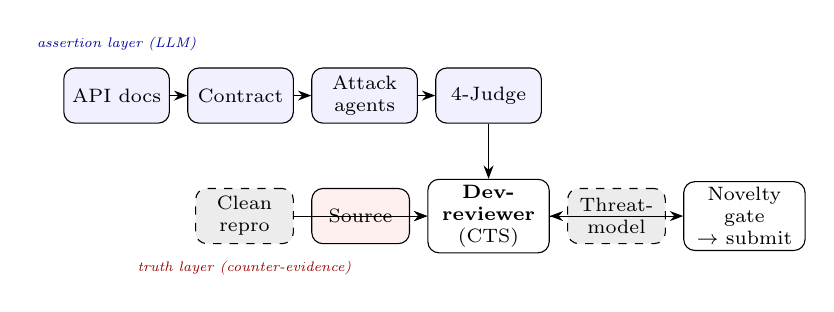
\begin{tikzpicture}[
  node distance=2.2mm and 2.2mm,
  font=\scriptsize,
  assert/.style={draw, rounded corners, fill=blue!6, align=center, inner sep=2pt, text width=12mm, minimum height=7mm},
  truth/.style={draw, rounded corners, fill=red!6, align=center, inner sep=2pt, text width=11mm, minimum height=7mm},
  truthunval/.style={draw, rounded corners, dashed, fill=gray!15, align=center, inner sep=2pt, text width=11mm, minimum height=7mm},
  gate/.style={draw, rounded corners, align=center, inner sep=2pt, text width=14mm, minimum height=7mm},
  arr/.style={-Stealth, thin}
]
\node[assert] (docs) {API docs};
\node[assert, right=of docs] (contract) {Contract};
\node[assert, right=of contract] (attack) {Attack\\agents};
\node[assert, right=of attack] (judge) {4-Judge};
\node[gate, below=7mm of judge] (devrev) {\textbf{Dev-reviewer}\\\scriptsize(CTS)};
\node[truth, left=of devrev] (src) {Source};
\node[truthunval, left=of src] (repro) {Clean\\repro};
\node[truthunval, right=of devrev] (tm) {Threat-\\model};
\node[gate, right=of tm] (out) {Novelty gate\\$\to$ submit};
\draw[arr] (docs)--(contract);
\draw[arr] (contract)--(attack);
\draw[arr] (attack)--(judge);
\draw[arr] (judge)--(devrev);
\draw[arr] (repro)--(devrev);
\draw[arr] (src)--(devrev);
\draw[arr] (tm)--(devrev);
\draw[arr] (devrev)--(out);
\node[font=\tiny\itshape, color=blue!60!black] at ($(docs.north)+(0,3mm)$) {assertion layer (LLM)};
\node[font=\tiny\itshape, color=red!60!black] at ($(repro.south)+(0,-3mm)$) {truth layer (counter-evidence)};
\end{tikzpicture}
\caption{TestVDB pipeline. The assertion layer (LLM contract + 4-judge) is falsified by the dev-reviewer's three counter-evidence anchors (truth layer): the source anchor is validated in our retrospective, while the reproduction and threat-model anchors (gray, dashed) are design-level and not yet evaluated. CTS = Contract-Truth Separation.}
\label{fig:overview}
\end{figure}

\subsection{Contract Extraction and the Threat-Model Prior}\label{sec:tm}
A knowledge-extractor agent crawls official API documentation and emits structured contracts (parameter domains, enum values, documented limits, status-code semantics) that seed both attack agents and judges. A threat-model artifact encodes recurring by-design intents (idempotency, eventual consistency, lenient defaults) and known blind spots. It is \emph{designed} to be injected at generation, judgment, and dedup; however, in our runs the blindspot indicators were never populated and its effect could not be isolated (Section~\ref{sec:eval-tm}), so we treat it as an unvalidated optional prior rather than a working component of the evaluated system.

\subsection{Attack Generation and the Four-Judge Debate}
Three attack agents target the compliance dimensions: a \emph{boundary} agent (illegal-success at parameter, enum, and limit edges---the dominant yield), a \emph{semantic} agent (diagnostic-quality violations), and a \emph{state} agent (state/logic inconsistencies). Candidates enter a four-judge debate (evidence/severity/novelty/doc axes) drawing on multi-agent verification ideas~\cite{du2023improving}. The Stage-2 output of this debate feeds the dev-reviewer.

\subsection{Contract-Truth Separation and the Dev-Reviewer}\label{sec:cts}
Single-layer LLM judgment is unreliable because the same model family generates the contract and judges compliance. CTS breaks this self-confirmation by introducing an independent truth layer. The dev-reviewer agent proxies maintainer authority and falsifies each Stage-2 candidate along three anchors:
\begin{itemize}[leftmargin=*,itemsep=2pt]
\item \textbf{Clean reproduction.} Build a minimal reproducer against a live VDBMS of the pinned target version; reject candidates whose ``defect'' is a tooling artifact (we withdrew early candidates that misread a missing \texttt{rowCount} field as ``returns $-1$'').
\item \textbf{Source-grounded verification.} Locate the implementation behind the API and check whether the observed behavior is intended---the direct counter to contract hallucination (Section~\ref{sec:hallucination}).
\item \textbf{Threat-model cross-check.} Match against known by-design intents before flagging a violation.
\end{itemize}
This mirrors maintainer adjudication: most of our false positives stem from contracts stricter than true intent, and source grounding is what exposes them.

\subsection{Novelty Gate}
A two-layer gate prevents re-reporting: L1 checks local history and the threat-model blind-spot set; L2 queries the target repository's issues and PRs. Candidates surviving both are submitted.

%=========================================================================
\section{Contract Hallucination Propagation}\label{sec:hallucination}
We highlight a phenomenon that, to our knowledge, has not been characterized in LLM-driven testing. When an LLM generates the contract \emph{and} judges compliance, hallucinated constraints are not caught by the judge---they are produced by the same generation--judgment family and thus inherit mutual confirmation. We observed two forms.

\textbf{(1) Fabricated provenance.} The formalizer produced a ``complexity requirement'' attributed to \texttt{constant.go}; source grounding showed the constant guards a past performance regression, not a behavioral constraint. The Stage-2 judge nonetheless confirmed violations against it.

\textbf{(2) Over-strict intent.} 12 of the 48 substantively adjudicated submissions (25\%) were marked by-design: the contract demanded rejection of behaviors maintainers intended to allow---idempotent duplicate creates returning success, eventual-consistency staleness, lenient naming defaults, and silent enum/empty substitutions.

Formally, let $C_{\mathrm{LLM}}$ be the LLM-derived contract and $C_{\mathrm{true}}$ the maintainer intent. Single-layer judgment assumes $C_{\mathrm{LLM}} = C_{\mathrm{true}}$; when $C_{\mathrm{LLM}} \supset C_{\mathrm{true}}$ (stricter), genuine by-design behaviors are flagged as violations, and the judge---sharing the generator's bias---does not dissent. The dev-reviewer's source-grounded anchor is the mitigation: it reintroduces an external truth signal ($C_{\mathrm{true}}$ proxied by source and history). We present this as a qualitative characterization; a quantitative study of hallucination frequency is future work, and the 12 by-design cases are direct observations rather than a measured rate over all inputs.

%=========================================================================
\section{Evaluation}\label{sec:eval}

We address three primary research questions (RQ1--RQ3) and report one exploratory negative result (RQ4, Section~\ref{sec:eval-tm}).

\subsection{RQ1: Detection Capability}
We ran TestVDB against five VDBMSs, pinning exact target versions. Table~\ref{tab:yield} reports the yield.

\begin{table}[t]
\caption{Issues submitted and maintainer outcomes (5 VDBMSs). 52 of the 111 submissions have been adjudicated (36 acknowledged $=$ 28 fixed $+$ 8 accepted, 12 by-design, 4 rejected). Of the remaining 59, 30 are \emph{pending} (open, awaiting triage) and drive the sensitivity interval in Section~\ref{sec:eval-rq3}; 29 are \emph{excluded} (closed-no-label or duplicate, unresolvable) and lie outside that interval.}
\label{tab:yield}
\small
\begin{tabular}{lrrrrrrr}
\toprule
VDBMS & Sub. & Fix. & Acc. & ByD. & Rej. & Pend. & Excl. \\
\midrule
Milvus      & 51 & 14 & 8 & 12 & 0 & 0  & 17 \\
Qdrant      & 26 & 11 & 0 & 0  & 3 & 8  & 4 \\
Weaviate    & 30 & 3  & 0 & 0  & 1 & 21 & 5 \\
MeiliSearch & 3  & 0  & 0 & 0  & 0 & 0  & 3 \\
Chroma      & 1  & 0  & 0 & 0  & 0 & 1  & 0 \\
\midrule
\textbf{Total} & \textbf{111} & \textbf{28} & \textbf{8} & \textbf{12} & \textbf{4} & \textbf{30} & \textbf{29} \\
\bottomrule
\end{tabular}
\end{table}

\paragraph{Defect-type distribution.} Of the 36 acknowledged true positives, 27 (75\%) are boundary/validation, 3 (8\%) diagnostic-quality, 2 (6\%) state/logic, 1 (3\%) crash, and 3 (8\%) result-correctness. The result-correctness cases are instructive: they include \texttt{COSINE} distance returning $>1.0$ for identical vectors (a hard mathematical-invariant violation, reproduced on both Milvus and Qdrant), incomplete index results (2 of 25 matching points returned), and a payload filter returning points with a missing field. These are detectable because they violate expressible invariants; soft result-correctness (ANN recall/ranking error) remains open.

\paragraph{Complementarity with VDBFuzz.} Our yield is almost entirely non-crash (35/36); VDBFuzz's crash oracle---its title frames the problem as ``Crash Bugs''~\cite{vdbfuzz26} and its source contains no compliance-checking logic---cannot detect non-crash defects, so at most 1/36 of our yield (the single crash case) could overlap with VDBFuzz's targets. Conversely, our L1 gate deliberately filters crash-prone inputs, so TestVDB does not target the crash bugs VDBFuzz finds. The complementarity follows from the oracle definitions; a head-to-head empirical comparison on identical targets is future work.

\subsection{RQ2: Case Studies}
We trace three end-to-end cases that span the TP/FP boundary and the dev-reviewer's role, then isolate a model-free oracle subclass.
\textbf{True positive, correctly surfaced (Milvus \#47729).} An invalid \texttt{nprobe}=0 was accepted by search. The attack agent derived the probe from the contract; the four-judge debate confirmed it; the dev-reviewer's source anchor raised no counter-evidence (no documented lower bound); the maintainer fixed it.
\textbf{True positive, correctly surfaced (Milvus \#49844).} An empty filter silently triggered a full scan; same path; maintainer accepted.
\textbf{False positive, correctly suppressed (Milvus \#50193).} \texttt{get\_stats} returned \texttt{rowCount}=0 immediately after insert. The four-judge confirmed it as a bug; the dev-reviewer's source anchor reclassified it as documented eventual consistency (async aggregation; 0 is a valid intermediate)---precisely the consistency-semantics FP class the source anchor targets---and the maintainer later closed it as by-design, confirming the reclassification.
\textbf{Model-free mathematical-invariant oracle (Milvus \& Qdrant).} The \texttt{COSINE} distance returned $>1.0$ for identical vectors, independently reproduced on both systems. Unlike the cases above, this violates a \emph{mathematical invariant} (cosine similarity is bounded in $[-1,1]$) and needs no LLM judgment---an expressible, model-free oracle subclass worth distinguishing from contract oracles. The same class catches incomplete index results (2/25 matching points returned) and payload filters returning points with a missing field.

\subsection{RQ3: Precision --- Controlled Retrospective and Aggregate}\label{sec:eval-rq3}

\paragraph{Controlled retrospective (primary, same population).} We re-triaged all 52 maintainer-adjudicated candidates (36 TP, 16 FP) under two blind conditions on the \emph{same} population: claim-only (the 4-judge layer) vs.\ source-grounded (the dev-reviewer's source anchor), outcomes hidden via label-isolated agents. Source-grounding lifts FP suppression from 5/16 ($31\%$) to 13/16 ($81\%$, $2.6\times$)---Milvus $33\%{\to}75\%$, non-Milvus $0\%{\to}100\%$---while retaining 29/30 TPs ($96.7\%$, $n{=}30$; 6 TPs were unreachable due to API rate limits). This is the same-population comparison we rely on for the dev-reviewer's contribution. (An earlier Milvus v2.6.19 ablation batch showed the dev-reviewer removing 26/33 FPs ($79\%$); we report this as directional support rather than a lift, because that batch's candidate composition is not cleanly comparable to the single-layer baseline.)

\paragraph{Aggregate maintainer-adjudicated precision.} Across all five VDBMSs, 52 of the 111 submissions have been adjudicated (36 acknowledged, 12 by-design, 4 rejected). Counting by-design and rejected as maintainer-judged false positives, aggregate precision is
\[
\mathrm{precision}_{\mathrm{adj}} = \frac{\mathrm{acknowledged}}{\mathrm{acknowledged}+\mathrm{by\text{-}design}+\mathrm{rejected}} = \frac{36}{36+12+4} = 69.2\%.
\]
We report this as an end-to-end operating point, \emph{not} as the ``after'' arm of the ablation ratio above, because it is measured on a different population (five libraries) and denominator (adjudicated submissions).

\paragraph{Sensitivity to pending submissions.} Of the 59 submissions not yet adjudicated, 30 are pending (open, awaiting triage) and 29 are excluded (closed-no-label or duplicate, unresolvable); the sensitivity below addresses only the 30 pending, and the 29 excluded lie outside it. Because maintainers may triage obvious bugs first, excluding pending items can bias precision upward. Bounding both extremes: resolving all 30 pending as valid gives $(36{+}30)/(52{+}30)=80.5\%$; resolving all as invalid gives $36/82=43.9\%$. Aggregate precision therefore lies in $[43.9\%, 80.5\%]$, with $69.2\%$ as the adjudicated-only point estimate. We report the interval rather than the point estimate alone to make the selection effect explicit.

\paragraph{Within-system baseline.} The claim-only condition above (simulating a single-layer 4-judge pipeline without the dev-reviewer) lets 11/16 FPs through as judged-TPs, for a judgment-layer precision of 33/44 $=$ 75\%; the source-grounded condition lets only 3/16 FPs through (29/32 $=$ 91\%).\footnote{The two conditions use different TP bases: claim-only scored all 36 TPs (retaining 33), while source-grounding scored the 30 reachable via the GitHub API (retaining 29, with 6 TPs rate-limited); the comparison is within the same 52-candidate population but across slightly different TP denominators.} This isolates the dev-reviewer's contribution within the same 52-candidate pool. We do \emph{not} have an end-to-end \emph{external} baseline (heuristic or human); the single-layer counterfactual next provides the end-to-end single-layer arm, but re-submitting a fresh single-layer cohort for independent maintainer triage remains future work.

\paragraph{Single-layer counterfactual: precision lift without recall cost.} Removing the FP-suppression chain and re-running generation plus the four-judge debate on milvus v2.6.19 yields a single-layer arm. A fresh round of 15 attack probes, adjudicated by the same four-judge debate, confirmed 3 candidates: 2 true positives acknowledged by maintainers (invalid \texttt{nprobe}=0, \texttt{milvus-io/milvus}\,\#47729; empty-filter full scan, \#49844) and 1 false positive maintainers classify as by-design eventual consistency (\texttt{get\_stats} \texttt{rowCount}=0, \#50193)---precisely the consistency-semantics FP class the suppression layer targets. Blindly re-adjudicating the dev-reviewer's 27 killed candidates (5-batch LLM adjudication + 7 live re-probes on v2.6.19, two of which overturned the LLM's initial TP) confirms all 27 as true false positives: \emph{dev-reviewer precision $27/27$, over-kill $0/27$}. End-to-end, the single layer would submit every four-judge-confirmed candidate; combining the 27 suppressed (all FP) with the $36/52$ TestVDB baseline gives single-layer precision $36/(36{+}16{+}27) = 45.6\%$, versus TestVDB's $69.2\%$---a $+23.7$\,pp lift from FP-suppression at zero recall cost. FP-suppression's precision advantage is therefore not bought with lost bugs.

\paragraph{Anchor attribution.} The dev-reviewer's three counter-evidence anchors contribute asymmetrically. Measured on the 16 FPs, adding the \emph{source} anchor to the claim-only layer drives the full lift above: claim-only suppresses 5/16 ($31\%$); adding source reaches 13/16 ($81\%$, $2.6\times$). The 3 residual misses are \emph{silent-absent} cases---no validation code exists to cite, so the agent defaults to ``bug''---which are exactly what the \emph{threat-model} anchor is designed to catch; its blindspot indicators were never populated (\S\ref{sec:eval-tm}), so those 3 leak. The \emph{reproduction} anchor requires a live VDB container and is not exercised in this retrospective. We therefore attribute the measured $81\%$/$96.7\%$ to the source anchor alone, treating reproduction and threat-model anchors as unmeasured future components---a gap we flag rather than disguise.

\paragraph{Contract coverage (upstream extraction).} Full end-to-end discovery recall would require running TestVDB against bug-present old versions, whose API docs are often no longer available (e.g., Milvus 2.2/2.3). As a partial probe we measure the upstream precondition: can the knowledge-extractor derive, from current docs, a contract that catches a known historical violation? On 9 held-out pre-2024 compliance bugs (Milvus/Qdrant/Weaviate, excluding our own submissions; chosen pre-2024 to limit LLM training leakage), a blind judge found current docs cover 6/9 violations' contracts ($67\%$); the 3 misses are genuine contract gaps (unrecognized query params; diagnostic-quality requirements; and one case where the judge mistook the buggy validation itself for the contract---a limitation of using LLM knowledge as a doc proxy). This measures only the extraction upstream, not full-pipeline discovery (attack generation and judging are not exercised); establishing true discovery recall against bug-present versions is future work.

\subsection{RQ4 (Exploratory, not a contribution): Threat-Model Prior}\label{sec:eval-tm}
We ran a double-blind ablation on Milvus v2.6.17 (control with threat-model cognition vs.\ experiment without; $n{=}5$ TP, 7 FP). TP recall moved 20\%/60\% (control/experiment); FP-correct 86\%/57\%. We report this as an \emph{exploratory negative result}: blindspot indicators were never populated, the dev-reviewer was unstable across runs (2/2 CONFIRMED/FP), and $n{=}5$ is below significance. We emphasize these 20\%/60\% figures are the TM control/experiment split, \emph{not} a stable estimate of dev-reviewer TP recall: the controlled retrospective (\S\ref{sec:eval-rq3}) measures the latter at $96.7\%$ ($n{=}30$), i.e., the dev-reviewer's source anchor does not trade away TP recall.

\subsection{Threats to Validity}
\emph{Internal:} maintainer acknowledgment is a weak ground truth. \emph{External:} the same-population ablation (RQ3) is Milvus-plus-Qdrant only; Weaviate submissions are undiagnosed and excluded from precision estimates. \emph{Construct:} defect-type classification is title-based, pending per-defect confirmation. \emph{LLM variance:} re-adjudicating the 46 source-grounded candidates five times with independent agents yields $99.1\%$ pairwise agreement and $45/46$ unanimous verdicts---judgment-layer noise is near-zero; residual variance sits upstream in version-pinned source extraction. \emph{Recall scope:} the $96.7\%$ figure is judgment-layer TP retention, not end-to-end discovery recall (future work). \emph{Single-layer counterfactual:} the $27$ killed labels are blind-LLM-adjudicated plus live re-probe ($7/27$); the $45.6\%$ single-layer figure mixes this proxy ground truth with the maintainer-adjudicated $36/52$ baseline and is bounded to one feedback cycle.

%=========================================================================
\section{Related Work}\label{sec:rw}
\paragraph{VDBMS testing.} VDBFuzz~\cite{vdbfuzz26} is the first dedicated VDBMS fuzzer (crash-oracle-based) and is complementary to this work. The roadmap~\cite{roadmap25} and the empirical bug study~\cite{bugstudy25} define the agenda and taxonomy we build upon. MeTMaP~\cite{metmap24} applies metamorphic testing to false vector matching in LLM-augmented generation. BUZZBEE~\cite{buzzbee24} fuzzes general DBMSs.
\paragraph{REST API and schema testing.} RESTler~\cite{restler19} infers producer--consumer dependencies among REST request types for stateful fuzzing; EvoMaster~\cite{evomaster21} evolves REST API test sequences. These target schema-conformance and crash at the API boundary; we extend the boundary to \emph{semantic} compliance (does the response honor the documented contract?) and to VDBMS-specific invariants.
\paragraph{Database correctness oracles.} NoREC~\cite{norec20} tests SQL via a non-optimizing reference engine; TLP~\cite{tlp20} partitions queries three ways; DQE~\cite{dqe20} pivots query execution; DDLCheck~\cite{ddlcheck25} targets DDL correctness. These assume reference SQL semantics absent in VDBMS APIs; our contract oracle replaces reference SQL with documentation-derived invariants.
\paragraph{LLM-based testing and verification.} LLMs increasingly drive test generation and software-engineering tasks~\cite{hou23llmse}; we use multi-agent debate~\cite{du2023improving} for generation and judgment. The contract-hallucination failure mode we identify is a spec-extraction instance of LLM hallucination more broadly~\cite{ji23hall}, mitigated in general by self-consistency~\cite{wang22sc}---we instantiate the mitigation as source-grounded falsification rather than prompt-level consensus.
\paragraph{Test oracles and contracts.} The oracle problem is a long-standing concern~\cite{barr15}; our contract oracle is an instance of the \emph{specified} class and the cosine-bounded / completeness subclass is an instance of the \emph{derivable} class. Property-based testing~\cite{claessen00} and Design by Contract~\cite{meyer92dbc} are precursors of specification-driven checking; static API-misuse detection~\cite{amann19} targets client-side misuse, whereas we target server-side non-compliance. General fuzzing is surveyed in~\cite{manes21}.

%=========================================================================
\section{Conclusion and Future Work}\label{sec:conc}
We presented TestVDB, the first LLM-driven system for detecting API compliance defects in VDBMSs, built on Contract-Truth Separation. On a controlled retrospective over 52 candidates, the dev-reviewer's source anchor lifts false-positive suppression from 31\% to 81\% while retaining 96.7\% of true positives; aggregated over five systems, maintainer-adjudicated precision is 69.2\% (within $[43.9\%, 80.5\%]$ under pending sensitivity). Contract hallucination propagation motivates the design. \emph{Scope:} TestVDB targets boundary/validation compliance and complements crash-focused fuzzing; it does not solve result-correctness oracles (ANN recall, ranking). Contract hallucination propagation generalizes beyond VDBMSs: any system where one LLM family both extracts a spec and checks compliance is susceptible, and CTS-style source-grounded falsification should extend to REST APIs and cloud services with documented contracts. Future work: stronger dev-reviewer backbones, an empirical VDBFuzz comparison on identical targets, cross-library ablation beyond Milvus and Qdrant, and an end-to-end discovery-recall study.

%=========================================================================
\bibliographystyle{ACM-Reference-Format}
\bibliography{references}

\end{document}
